\documentclass[11pt,letterpaper]{article}
\usepackage{fontspec}
\setmainfont{texgyrepagella}[Extension=.otf,UprightFont=*-regular,BoldFont=*-bold,ItalicFont=*-italic,BoldItalicFont=*-bolditalic]
\usepackage[bidi=default]{babel}
\babelprovide[import,main]{spanish}
\babelprovide[import]{hebrew}
\babelprovide[import]{ancientgreek}
\babelfont[hebrew]{rm}[Path=fonts/,BoldFont=NotoHebrewSerif-700.ttf,Scale=0.95]{NotoHebrewSerif-400.ttf}
\babelfont[ancientgreek]{rm}[Path=fonts/]{GFSPorson.otf}
\newcommand{\heb}[1]{\mbox{\foreignlanguage{hebrew}{#1}}}
\newcommand{\grc}[1]{\foreignlanguage{ancientgreek}{#1}}
\newcommand{\hebverso}[1]{\par\smallskip{\centering\begin{otherlanguage}{hebrew}\large #1\end{otherlanguage}\par}\smallskip}
\usepackage[margin=2.5cm,headheight=14pt]{geometry}
\usepackage{microtype,ragged2e,booktabs,graphicx,xcolor,csquotes,array}
\usepackage[hidelinks]{hyperref}\usepackage{xurl}\urlstyle{same}
\usepackage[most]{tcolorbox}
\usepackage{tikz}\usetikzlibrary{arrows.meta,positioning,calc,decorations.pathreplacing}
\usepackage{titlesec,fancyhdr,extramarks}
% Paleta "Israel": café ladrillo (ladrillos de Egipto, Éx 1:14), oro del santuario, piedra de Jerusalén
\definecolor{cafe}{RGB}{96,52,30}\definecolor{cafeosc}{RGB}{50,25,13}\definecolor{tinta}{RGB}{44,28,18}
\definecolor{oro}{RGB}{196,148,40}\definecolor{ladrillo}{RGB}{158,70,40}
\definecolor{piedra}{RGB}{240,228,203}\definecolor{sepia}{RGB}{104,86,62}
\titleformat{\section}{\Large\bfseries\color{ladrillo}}{\thesection.}{0.6em}{}
\titleformat{\subsection}{\large\bfseries\color{cafe}}{\thesubsection}{0.6em}{}
\pagestyle{fancy}\fancyhf{}
\fancyhead[L]{\foreignlanguage{spanish}{\small\itshape\color{sepia}\firstleftmark}}\fancyhead[R]{\foreignlanguage{spanish}{\small\color{sepia}\thepage}}
\renewcommand{\sectionmark}[1]{\markboth{#1}{}}
\setlength{\parindent}{1.27cm}\linespread{1.15}\setlength{\emergencystretch}{3em}
\newtcolorbox{cita}[1][]{enhanced,colback=piedra,colframe=ladrillo!85!oro,boxrule=0pt,leftrule=2.5pt,arc=0pt,
  left=8pt,right=8pt,top=5pt,bottom=5pt,before skip=8pt,after skip=8pt,fontupper=\itshape,#1}
\newcommand{\fuente}[1]{\par\hfill{\upshape\bfseries\small\textcolor{ladrillo}{#1}}}
\newtcolorbox{nota}[1][]{enhanced,colback=oro!12,colframe=oro!80!ladrillo,boxrule=0.6pt,arc=2pt,
  fonttitle=\bfseries\small,coltitle=cafe,colbacktitle=oro!35,fontupper=\small,title={#1}}
\newcommand{\refapa}[1]{\par{\RaggedRight\hangindent=1.27cm\hangafter=1\noindent #1\par}\vspace{4pt}}
\newcommand{\destacar}[1]{\textbf{\textcolor{ladrillo}{#1}}}
\title{\color{ladrillo}\bfseries De Abraham al Éxodo\\[4pt]\large\color{cafe}\mdseries Un pueblo creado desde la imposibilidad, llamado a bendecir y sostenido por una promesa de regreso}
\author{}\date{\color{sepia}Serie «Israel, el pueblo de Dios» · Estudio 1}
\begin{document}
\maketitle\thispagestyle{empty}

\begin{abstract}\noindent
Este primer estudio de la serie recorre la historia de Israel desde el llamado de Abram (Gn 12) hasta la salida de Egipto y el cántico del mar (Éx 15). Sostiene que Israel debe su existencia a una palabra de Dios dirigida a una pareja estéril, y no a la fuerza de una etnia, y que desde ese origen lleva consigo una vocación hacia las naciones que el Sinaí formulará como «reino de sacerdotes y nación santa» (Éx 19:6). Sostiene también que la promesa de restauración no es un recurso tardío de los profetas: está inscrita ya en el pacto con Abraham, que anuncia de antemano un destierro y un regreso (Gn 15:13–16). Para ello se reúnen el texto hebreo, los datos arqueológicos sobre semitas en Egipto con sus límites, la memoria litúrgica judía (la Amidá, la Hagadá de Pésaj, el shofar de Rosh Hashaná) y la lectura que Isaías, Jeremías y Pablo hacen de Abraham y del Éxodo. El recorrido muestra que la memoria del pacto por la que Dios «se acordó de su pacto con Abraham, con Isaac y con Jacob» (Éx 2:24) es la misma por la que, según Pablo, Israel sigue siendo «amado por causa de los padres» (Ro 11:28).
\par\smallskip\noindent\textbf{Palabras clave:} Abraham, pacto, Éxodo, remanente, restauración, Isaías, Jeremías, Romanos 11.
\end{abstract}

\section{Introducción}

Que Dios haya elegido un pueblo es una idea que incomoda. Al lector moderno le suena a favoritismo; a muchos cristianos, a un andamio provisional que se retiró una vez levantada la iglesia. Pablo la entiende de otra manera: los israelitas siguen siendo aquellos «de quienes son la adopción, la gloria, los pactos, la promulgación de la ley, el culto y las promesas; de quienes son los padres» (Ro 9:4–5), y «los dones y el llamamiento de Dios son irrevocables» (Ro 11:29). Una afirmación así solo se comprende si se vuelve al principio, a Abraham.

Lo que allí se descubre es, ante todo, que Israel es obra de Dios y no conquista humana: nace de Sara, que era estéril (Gn 11:30), y de una promesa que Abraham no llegó a ver cumplida (Hch 7:5). Y se descubre, además, que el ciclo de destierro y regreso acompaña a este pueblo desde antes de que exista, porque Dios anuncia que la descendencia de Abram será extranjera y oprimida, y que «en la cuarta generación volverán acá» (Gn 15:16). Cuanto los profetas digan más tarde sobre Babilonia y la dispersión no hará sino ampliar ese primer trazo.

\begin{center}\small
\renewcommand{\arraystretch}{1.3}
\begin{tabular}{>{\RaggedRight\arraybackslash}p{3.1cm}>{\RaggedRight\arraybackslash}p{5.6cm}>{\RaggedRight\arraybackslash}p{5.2cm}}
\toprule
\textbf{Eje de la serie} & \textbf{Pregunta en esta etapa} & \textbf{Textos centrales}\\
\midrule
Nación santa y reino de sacerdotes & ¿Para qué fue llamado Abraham y qué función tiene su descendencia ante las naciones? & Gn 12:1–3; 18:18–19; 22:18; Éx 4:22; 19:4–6\\
Promesa de restauración & ¿Dónde aparece por primera vez el patrón de exilio y regreso, y en qué se funda? & Gn 15:13–16; 46:3–4; 50:24–25; Éx 2:24; 6:6–8\\
Proyección profética y paulina & ¿Cómo releen Isaías, Jeremías y Pablo a Abraham y al Éxodo? & Is 41:8; 51:1–3; Jer 31:35–37; 33:25–26; Ro 4; 11:16, 28–29\\
\bottomrule
\end{tabular}\end{center}

\begin{nota}[Sobre traducción, numeración y fechas]
Las citas bíblicas son traducción propia desde el texto hebreo (BHS) y griego (NA28); la Septuaginta se cita según Rahlfs-Hanhart. Cuando la numeración hebrea difiere de la española, se da la española y la hebrea entre corchetes, por ejemplo Gn 32:28 [32:29]. Las fechas se indican como a.\,e.\,c. (antes de la era común) y e.\,c.
\end{nota}

\section{Marco cronológico}

Para fechar el período, la Biblia ofrece dos datos. Según 1~R 6:1, la salida de Egipto ocurrió 480 años antes del cuarto año de Salomón; si ese año se sitúa hacia el 966 a.\,e.\,c., el Éxodo caería hacia el 1446 a.\,e.\,c. («datación temprana»). Éx 12:40, por su parte, da 430 años de permanencia. Muchos historiadores prefieren una «datación tardía», en el siglo \textsc{xiii} a.\,e.\,c., porque Éx 1:11 menciona la ciudad de Ramsés, que suele identificarse con Pi-Ramsés (Qantir), construida bajo Ramsés~II (Hoffmeier, 1997; Kitchen, 2003). Quienes defienden la fecha temprana responden que el nombre pudo actualizarse durante la transmisión del texto, como sucede con «Dan» en Gn 14:14. El debate sigue abierto y no se zanjará aquí: para el argumento basta la secuencia de los hechos, no el año exacto.

\begin{nota}[Precisión textual: los 430 años de Éx 12:40]
El Texto Masorético dice que Israel habitó en Egipto 430 años. La Septuaginta y el Pentateuco samaritano leen «en la tierra de Egipto \emph{y en la tierra de Canaán}», de modo que los 430 años cubren también la etapa de los patriarcas. Pablo cuenta 430 años desde la promesa hasta la ley (Gá 3:17), lo que concuerda con la lectura larga. Flavio Josefo da 215 años en Egipto (\emph{Antigüedades} 2.15.2), y la cronología rabínica tradicional cuenta los 400 años de Gn 15:13 desde el nacimiento de Isaac y deja unos 210 años en Egipto (Seder Olam Rabbah; Rashi sobre Éx 12:40; Guggenheimer, 1998). Este estudio sigue el TM en la traducción y señala la lectura alternativa.
\end{nota}

\begin{center}
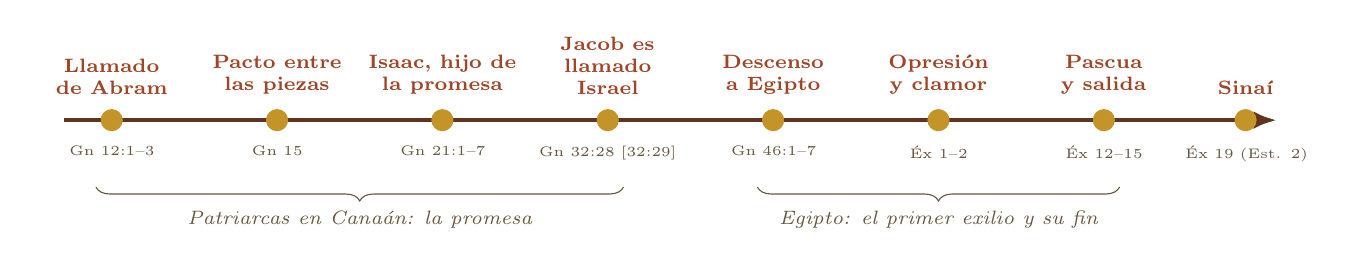
\begin{tikzpicture}[x=1cm,y=1cm]
\draw[line width=1.6pt,cafe,-{Latex[length=3mm]}] (0,0) -- (15.4,0);
\foreach \x/\t/\b in {0.6/{Llamado de Abram}/{Gn 12:1--3},
                      2.7/{Pacto entre las piezas}/{Gn 15},
                      4.8/{Isaac, hijo de la promesa}/{Gn 21:1--7},
                      6.9/{Jacob es llamado Israel}/{Gn 32:28 [32:29]},
                      9.0/{Descenso a Egipto}/{Gn 46:1--7},
                      11.1/{Opresión y clamor}/{Éx 1--2},
                      13.2/{Pascua y salida}/{Éx 12--15},
                      15.0/{Sinaí}/{Éx 19 (Est. 2)}}{
  \fill[oro] (\x,0) circle (4pt);
  \node[above,font=\scriptsize\bfseries,text=ladrillo,text width=1.9cm,align=center] at (\x,0.2) {\t};
  \node[below,font=\tiny,text=sepia,text width=1.8cm,align=center] at (\x,-0.2) {\b};}
\draw[decorate,decoration={brace,amplitude=5pt,mirror},sepia] (0.4,-0.85) -- (7.1,-0.85) node[midway,below=5pt,font=\scriptsize\itshape]{Patriarcas en Canaán: la promesa};
\draw[decorate,decoration={brace,amplitude=5pt,mirror},sepia] (8.8,-0.85) -- (13.4,-0.85) node[midway,below=5pt,font=\scriptsize\itshape]{Egipto: el primer exilio y su fin};
\end{tikzpicture}\\[2pt]
{\footnotesize\color{sepia}\textit{Nota.} Elaboración propia. Secuencia narrativa; las fechas absolutas están en debate (véase el texto).}
\end{center}

\section{Contexto histórico y arqueológico}

\subsection{De Ur a Harán y a Canaán}
Gn 11:31 hace salir a Taré y a Abram «de Ur de los caldeos» hacia Harán. Ur, en el sur de Mesopotamia, fue excavada por Leonard Woolley entre 1922 y 1934 y era una de las grandes ciudades de su tiempo. El calificativo «de los caldeos» refleja la denominación de una época posterior, cuando los caldeos dominaban la región; una tradición judía e islámica antigua prefiere identificar Ur con Urfa, en el norte, cerca de Harán (Sarna, 1989). Harán sí está bien atestiguada como centro de culto a la luna, igual que Ur, y ese dato ilumina Jos 24:2: «vuestros padres habitaron antiguamente al otro lado del río\ldots\ y servían a otros dioses». Cuando Abram deja su tierra, deja también los dioses de su padre.

\begin{center}\begin{minipage}{\linewidth}\centering
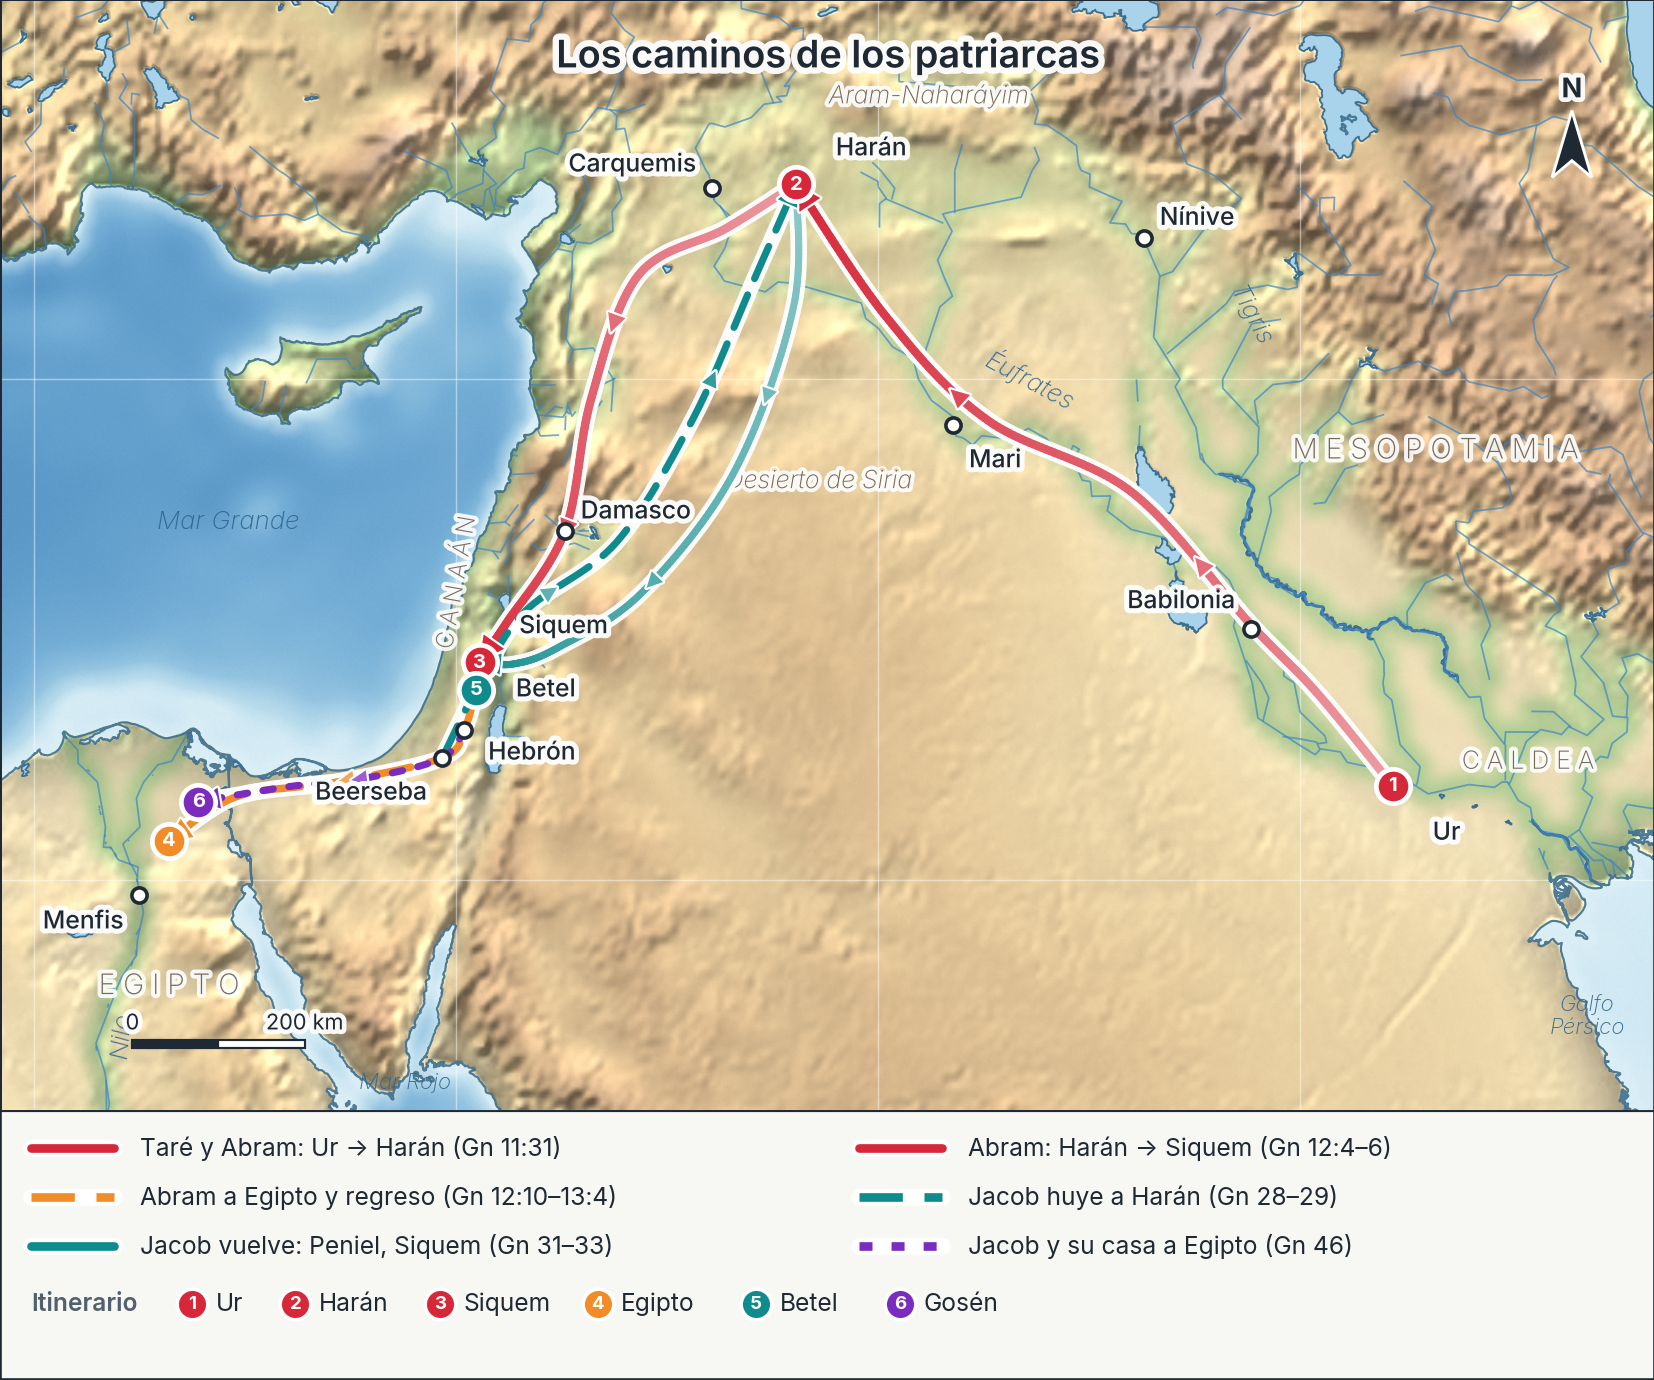
\includegraphics[width=1\linewidth]{mapa_patriarcas.png}\\[2pt]
{\footnotesize\color{sepia}\textit{Nota.} Elaboración propia: costas, lagos y ríos GSHHS/WDB y relieve sombreado (Basemap); ubicaciones antiguas aproximadas. }
\end{minipage}\end{center}


\subsection{Los patriarcas y el debate sobre su historicidad}
A mediados del siglo \textsc{xx} se citaban costumbres de los archivos de Nuzi y Mari (adopción, herederos sustitutos, nombres amorreos) como paralelos que situarían a los patriarcas en el Bronce Medio. Thompson (1974) y Van Seters (1975) mostraron que muchos de esos paralelos eran débiles o también tardíos, y una parte de la academia concluyó que los relatos no pueden fecharse. Otros autores sostienen que los nombres, los precios de esclavos y las formas de pacto encajan mejor en el segundo milenio que en el primero (Kitchen, 2003). Conviene separar las dos cuestiones. La arqueología no ha encontrado a Abraham, y difícilmente podría esperarse tal cosa de un pastor seminómada; el mundo que describe Génesis, en cambio, con sus migraciones de grupos semitas, sus pactos de tratado y sus descensos a Egipto en tiempos de hambre, resulta históricamente verosímil.

\begin{nota}[Precisión arqueológica: los camellos de Gn 12:16]
Gn 12:16 menciona camellos entre los bienes de Abram. Un estudio de restos óseos en el valle del Aravá sitúa la introducción del camello doméstico en el sur del Levante hacia el siglo \textsc{x} a.\,e.\,c. (Sapir-Hen y Ben-Yosef, 2013), y algunos lo leen como anacronismo. Otros recuerdan que la domesticación es anterior en Arabia y que un uso limitado por parte de grupos móviles no deja necesariamente huella en los asentamientos. La cuestión sigue en debate y no prueba nada en ninguna de las dos direcciones.
\end{nota}

\subsection{Semitas en Egipto}
En el período en que se sitúa a José y a la familia de Jacob, la presencia de semitas del Levante en Egipto era algo corriente, como muestran varios hallazgos:
\begin{itemize}
\item \textbf{Pintura de Beni Hasan} (tumba de Jnumhotep~II, c. 1890 a.\,e.\,c.): un grupo de 37 «asiáticos» (\emph{aamu}) encabezados por un jefe llamado Abisha llega a Egipto con mercancías, vestidos de colores (Newberry, 1893). No se trata de la familia de Jacob, pero la escena deja ver cómo eran estos grupos.
\item \textbf{Avaris} (Tell el-Dab\textquoteright a), en el delta oriental, zona de Gosén: las excavaciones de Manfred Bietak documentan desde c. 1800 a.\,e.\,c. una población de origen cananeo que creció hasta dar origen a la dinastía de los hicsos (Bietak, 1996).
\item \textbf{Papiro Brooklyn 35.1446}: una lista de siervos de una casa egipcia de fines del Reino Medio; cerca de la mitad tiene nombres semíticos del noroeste, entre ellos una mujer llamada \emph{Shifra}, el mismo nombre de una de las parteras de Éx 1:15 (Hayes, 1955; Albright, 1954). Nada indica que sea la misma persona; lo que el documento revela es que esos nombres eran habituales entre los semitas al servicio de casas egipcias.
\item \textbf{Estela de Merneptah} (c. 1208 a.\,e.\,c.): el faraón dice que «Israel está devastado; su descendencia no existe». Es la mención extrabíblica más antigua de Israel, y el escriba la acompaña del determinativo de pueblo, no del de territorio; hacia fines del siglo \textsc{xiii} a.\,e.\,c., por tanto, Israel ya era un pueblo identificable en Canaán.
\end{itemize}
Ninguna fuente egipcia narra el Éxodo, y con frecuencia se esgrime este silencio en su contra. Hoffmeier (1997) recuerda que las inscripciones reales egipcias no registraban derrotas y que la humedad del delta conserva muy mal los papiros; observa, además, que varios detalles del relato (nombres egipcios como Moisés, Putifar o Zafnat-panea, el trabajo con ladrillos y paja de Éx 5, la geografía del delta oriental) concuerdan con lo que se sabe de Egipto. La falta de evidencia directa pide cautela, pero no autoriza a negar el relato.

\section{Desarrollo bíblico}

\subsection{El llamado de Abram: un nombre recibido, no fabricado}
El llamado de Gn 12 llega justo después de Babel, donde los hombres dicen: «Hagámonos un nombre» (\heb{וְנַעֲשֶׂה־לָּנוּ שֵׁם}, Gn 11:4). A esa humanidad dispersa Dios responde con un hombre, a quien Él mismo promete engrandecer el nombre:

\hebverso{וְאֶעֶשְׂךָ לְגוֹי גָּדוֹל וַאֲבָרֶכְךָ וַאֲגַדְּלָה שְׁמֶךָ וֶהְיֵה בְּרָכָה\\
וַאֲבָרְכָה מְבָרְכֶיךָ וּמְקַלֶּלְךָ אָאֹר וְנִבְרְכוּ בְךָ כֹּל מִשְׁפְּחֹת הָאֲדָמָה}
\begin{cita}Haré de ti una nación grande, te bendeciré y engrandeceré tu nombre, y sé tú una bendición. Bendeciré a los que te bendigan, y al que te maldiga maldeciré; y en ti serán benditas todas las familias de la tierra.\fuente{(Gn 12:2--3)}\end{cita}

Los verbos están en primera persona («haré», «bendeciré», «engrandeceré»): la iniciativa pertenece por entero a Dios. Pero la «nación» (\heb{גּוֹי}, \emph{goy}) que promete no se agota en sí misma, porque el imperativo «sé una bendición» (\heb{וֶהְיֵה בְּרָכָה}, \emph{ve-heyé berajá}) le asigna una tarea, y esa tarea mira lejos: alcanza a «todas las familias de la tierra», las mismas que Gn 10 enumeró y Gn 11 dispersó. Dios escoge a uno para bendecir a todos, y esa lógica atraviesa la serie entera.

\begin{nota}[Precisión filológica: \emph{nivrejú}]
La forma \heb{וְנִבְרְכוּ} (\emph{ve-nivrejú}, nifal) puede entenderse como pasiva («serán benditas») o como reflexiva («se bendecirán», es decir, usarán tu nombre al bendecir). En Gn 22:18 y 26:4 aparece el hitpael \heb{וְהִתְבָּרְכוּ}, que favorece el sentido reflexivo. La Septuaginta tradujo en pasiva (\grc{ἐνευλογηθήσονται}), y Pablo sigue esa lectura en Gá 3:8. Con una u otra lectura, el destino de las naciones queda ligado a Abraham.
\end{nota}

\subsection{El pacto entre las piezas (Gn 15)}
Ningún capítulo pesa tanto en esta serie como Gn 15, y su punto de partida es la fe de Abram:

\hebverso{וְהֶאֱמִן בַּיהוָה וַיַּחְשְׁבֶהָ לּוֹ צְדָקָה}
\begin{cita}Y creyó a YHWH, y él se lo contó por justicia.\fuente{(Gn 15:6)}\end{cita}

El verbo \heb{הֶאֱמִן} (\emph{he'emín}, de la raíz \emph{'mn}, la misma de \emph{amén} y \emph{emuná}) significa apoyarse en alguien como en algo firme. Sobre este versículo levantará Pablo su argumento de Ro 4 y Gá 3.

Sigue el rito. Abram parte los animales, y Dios, en forma de «horno humeante y antorcha de fuego», pasa solo entre las mitades (Gn 15:17). En los tratados del antiguo Cercano Oriente, quien pasaba entre los animales partidos invocaba sobre sí la misma suerte si llegaba a romper el pacto, sentido que Jer 34:18–20 todavía conserva. Al pasar solo, Dios toma sobre sí toda la obligación. La tradición judía conoce el pasaje como \emph{berit bein ha-betarim}, «el pacto entre las piezas».

En medio del rito se oye, por primera vez en la Biblia, el anuncio de un exilio y de un regreso:

\hebverso{יָדֹעַ תֵּדַע כִּי־גֵר יִהְיֶה זַרְעֲךָ בְּאֶרֶץ לֹא לָהֶם וַעֲבָדוּם וְעִנּוּ אֹתָם אַרְבַּע מֵאוֹת שָׁנָה}
\begin{cita}Ten por cierto que tu descendencia será extranjera en una tierra que no es suya; los harán servir y los oprimirán cuatrocientos años. Pero también a la nación a la que servirán la juzgaré yo, y después de esto saldrán con gran riqueza [\ldots]. Y en la cuarta generación volverán acá.\fuente{(Gn 15:13--14, 16)}\end{cita}

El verbo de Gn 15:16 es \heb{יָשׁוּבוּ} (\emph{yashuvu}), de la raíz \heb{שׁוּב} (\emph{shuv}), «volver». Con ese mismo verbo se nombrarán el regreso del exilio y el arrepentimiento (\emph{teshuvá}), y con él expresará Israel su esperanza en adelante: Dt 30:3 («YHWH tu Dios hará volver tu cautividad»), Jer 29:14, Jer 31:16–17. Antes de que el pueblo exista, la secuencia ya está trazada: \destacar{promesa, destierro, juicio sobre el opresor, regreso}.

\subsection{Pacto perpetuo, nombre nuevo y circuncisión (Gn 17)}
En Gn 17 el pacto se llama \emph{perpetuo}:

\hebverso{וַהֲקִמֹתִי אֶת־בְּרִיתִי בֵּינִי וּבֵינֶךָ וּבֵין זַרְעֲךָ אַחֲרֶיךָ לְדֹרֹתָם לִבְרִית עוֹלָם}
\begin{cita}Estableceré mi pacto entre mí y ti, y tu descendencia después de ti, por sus generaciones, como pacto perpetuo.\fuente{(Gn 17:7)}\end{cita}

El nombre cambia de Abram a Abraham, explicado como «padre de una multitud de naciones» (\heb{אַב־הֲמוֹן גּוֹיִם}, \emph{av hamón goyim}, Gn 17:5). Pablo cita este versículo en Ro 4:17 para sostener que Abraham es padre de los creyentes de las naciones. La circuncisión, señal del pacto, queda grabada en la carne de la descendencia, aunque Moisés y los profetas dirán después que lo que Dios busca es circuncidar el corazón (Dt 10:16; 30:6; Jer 4:4).

\subsection{La Akedá: la promesa entregada y devuelta (Gn 22)}
Isaac nace contra toda posibilidad: Sara era estéril y ambos eran ancianos (Gn 18:11–14). Por eso resulta tan desconcertante que, en Gn 22, Dios pida a Abraham ofrecer precisamente al hijo en quien descansa la promesa. Abraham obedece, y Dios provee el carnero; el lugar recibe el nombre \heb{יְהוָה יִרְאֶה} (\emph{YHWH yiré}, «YHWH proveerá/verá», Gn 22:14). Dios renueva entonces la promesa con juramento: «en tu descendencia serán benditas todas las naciones de la tierra» (Gn 22:18). La tradición identifica el «monte Moriah» con el monte del templo, apoyada en 2 Cr 3:1; la carta a los Hebreos lee la escena como figura de resurrección (Heb 11:17–19).

\subsection{Jacob llamado Israel}
De Isaac la promesa pasa a Jacob por pura elección, sin mérito alguno de su parte, como subraya Pablo en Ro 9:10–13. En Peniel, Jacob lucha y recibe un nombre nuevo:

\begin{cita}No se dirá más tu nombre Jacob, sino Israel, porque has luchado con Dios y con los hombres, y has prevalecido.\fuente{(Gn 32:28 [32:29])}\end{cita}

El texto explica el nombre con el verbo \emph{sará}, «luchar»: \emph{Yisra-El}. Como tantas etimologías bíblicas, la explicación se apoya en el sonido de la palabra más que en su análisis lingüístico; gramaticalmente, el sentido más probable es «Dios lucha» o «que Dios prevalezca» (Sarna, 1989). Sea como fuere, el pueblo entero llevará el nombre de un hombre herido que no soltó a Dios hasta ser bendecido. En Gn 35:11 Dios le promete «una nación y un conjunto de naciones» (\heb{גּוֹי וּקְהַל גּוֹיִם}, \emph{goy u-qehal goyim}), y en Gn 48:19 Jacob dice que la descendencia de Efraín será «plenitud de las naciones» (\heb{מְלֹא־הַגּוֹיִם}, \emph{melo ha-goyim}). Esta última expresión reaparecerá cuando la serie llegue a la división del reino y a Romanos 11; por ahora basta con dejarla anotada.

\subsection{José y el primer remanente}
Con la historia de José la familia llega a Egipto. Cuando por fin se da a conocer a sus hermanos, José relee todo lo vivido como obra de la providencia:

\hebverso{לָשׂוּם לָכֶם שְׁאֵרִית בָּאָרֶץ וּלְהַחֲיוֹת לָכֶם לִפְלֵיטָה גְּדֹלָה}
\begin{cita}Dios me envió delante de vosotros para preservaros un remanente en la tierra y para daros vida por medio de una gran liberación.\fuente{(Gn 45:7)}\end{cita}

Es la primera vez que la palabra \heb{שְׁאֵרִית} (\emph{she'erit}, «remanente») se aplica a la familia de Israel. Isaías hará de ella una noción teológica central (Is 10:20–22), y Pablo la recogerá al escribir que «ha quedado un remanente escogido por gracia» (Ro 11:5). Llama la atención que este primer remanente no sobreviva solo para sí: gracias a José comen también Egipto y «toda la tierra» (Gn 41:57).

\subsection{Del descenso al Éxodo}
Antes del descenso, Dios habla a Jacob en Beerseba:

\hebverso{אָנֹכִי אֵרֵד עִמְּךָ מִצְרַיְמָה וְאָנֹכִי אַעַלְךָ גַם־עָלֹה}
\begin{cita}Yo descenderé contigo a Egipto, y yo también te haré subir de nuevo.\fuente{(Gn 46:4)}\end{cita}

Israel no desciende solo: su Dios baja con él al exilio. Al morir, José hace jurar a sus hermanos que llevarán sus huesos a la tierra, porque «Dios ciertamente os visitará» (\heb{פָּקֹד יִפְקֹד}, \emph{paqod yifqod}, Gn 50:24–25). Moisés cumplirá el juramento (Éx 13:19) y Hebreos lo cuenta como acto de fe (Heb 11:22).

El libro del Éxodo abre con un pueblo que se multiplica (Éx 1:7, eco de Gn 1:28), con la opresión del ladrillo y el barro (Éx 1:14) y con el clamor de los oprimidos. Si Dios responde, es por causa del pacto:

\hebverso{וַיִּזְכֹּר אֱלֹהִים אֶת־בְּרִיתוֹ אֶת־אַבְרָהָם אֶת־יִצְחָק וְאֶת־יַעֲקֹב}
\begin{cita}Y oyó Dios su gemido, y se acordó Dios de su pacto con Abraham, con Isaac y con Jacob.\fuente{(Éx 2:24)}\end{cita}

En hebreo, «acordarse» (\heb{זָכַר}, \emph{zajar}) es actuar a favor de alguien en virtud de un compromiso, mucho más que recuperar un dato olvidado. Desde la zarza, Dios encarga a Moisés que repita ante los ancianos las mismas palabras de José: \heb{פָּקֹד פָּקַדְתִּי} (\emph{paqod paqadti}, «ciertamente os he visitado», Éx 3:16). Una tradición midrásica dice que esa fórmula era la señal de redención transmitida desde José, por la cual los ancianos reconocerían al verdadero libertador (Pirqé de-Rabí Eliézer, cap. 48; Friedlander, 1916).

Antes de la primera plaga, Dios llama a Israel «mi hijo, mi primogénito» (\heb{בְּנִי בְכֹרִי יִשְׂרָאֵל}, Éx 4:22). En Éx 6:6–8 promete la liberación con una cadena de verbos: «os sacaré», «os libraré», «os redimiré», «os tomaré por pueblo», «os introduciré en la tierra». La Pascua (Éx 12) y el paso del mar (Éx 14–15) cumplen los cuatro primeros. Junto a Israel sale también «una multitud mixta» (\heb{עֵרֶב רַב}, \emph{érev rav}, Éx 12:38), de modo que ya en la primera redención hay gente de otras naciones que se suma al pueblo, y la ley de la Pascua contempla su incorporación (Éx 12:48–49).

\section{Israel como nación santa y reino de sacerdotes}

La fórmula de Éx 19:6, «vosotros me seréis un reino de sacerdotes y una nación santa» (\heb{מַמְלֶכֶת כֹּהֲנִים וְגוֹי קָדוֹשׁ}, \emph{mamléjet kohaním ve-goy qadosh}), se pronuncia en el Sinaí y ocupará el centro del Estudio~2, aunque su contenido se adelanta ya en la historia patriarcal. El sacerdote es un mediador que lleva a Dios ante el pueblo y al pueblo ante Dios, y esa mediación es justamente lo que ejercen los patriarcas:

\begin{itemize}
\item \textbf{Abraham edifica altares e invoca el nombre} de YHWH en cada etapa del camino (Gn 12:7–8; 13:18).
\item \textbf{Intercede por otros pueblos}: por Sodoma (Gn 18:22–33) y por Abimelec, rey filisteo, de quien Dios dice: «es profeta, y orará por ti» (Gn 20:7).
\item \textbf{Es elegido para enseñar}: «para que mande a sus hijos y a su casa después de sí que guarden el camino de YHWH, haciendo justicia y juicio» (Gn 18:19). Las naciones serán bendecidas a través de un pueblo que practique la justicia.
\item \textbf{José preserva la vida de las naciones} en la hambruna (Gn 41:57; 50:20).
\item \textbf{Israel es el primogénito} (Éx 4:22). En la familia antigua, el primogénito representaba a los hermanos y heredaba una función de liderazgo; en Israel los primogénitos fueron consagrados a Dios y luego sustituidos por los levitas (Éx 13:2; Nm 3:12). Si Israel es «primogénito», hay otros hijos, las naciones, y a ellos le corresponde representarlos.
\end{itemize}

El material de estudio de la congregación resume el llamamiento de Israel en cinco puntos: reino de sacerdotes y nación santa (Éx 19:6), luz para las naciones (Is 49:6), custodio de la palabra de Dios (Dt 4:5–8; Sal 147:19–20; Ro 3:1–2), testigo de la fidelidad de Dios (Is 43:10–12) y heredero de la tierra (Gn 13:14–15) (Departamento de Educación, s.\,f.). Los cinco están ya en germen en la etapa patriarcal.

Isaías volverá sobre el sacerdocio de Israel para situarlo al final de la restauración: «vosotros seréis llamados sacerdotes de YHWH; ministros de nuestro Dios os dirán» (\heb{וְאַתֶּם כֹּהֲנֵי יְהוָה תִּקָּרֵאוּ}, Is 61:6), e incluso lo abrirá a las naciones, de entre las cuales Dios tomará «sacerdotes y levitas» (Is 66:21). Pedro, por su parte, aplicará Éx 19:6 en su forma griega (\grc{βασίλειον ἱεράτευμα, ἔθνος ἅγιον}) a los creyentes de la diáspora (1~P 2:9). Leído a la luz de su origen, ese texto no deja a Israel de lado: muestra más bien a qué pueblo se incorporan los creyentes.

\section{Aporte de la tradición judía}

La memoria judía de esta etapa vive menos en los tratados que en la liturgia y el midrash, y al recorrerla conviene no confundir lo que dice el texto bíblico con lo que la tradición desarrolla a partir de él.

\subsection{Abraham en el midrash}
\begin{itemize}
\item \textbf{El rompedor de ídolos.} Bereshit Rabbah 38:13 cuenta que Abram, hijo de un fabricante de ídolos, rompió las imágenes del taller de su padre. La narración es haggádica y no pretende ser histórica, pero pone en escena lo que Jos 24:2 deja implícito: responder al llamado era abandonar la idolatría.
\item \textbf{«Abram el hebreo».} Gn 14:13 llama a Abram \heb{הָעִבְרִי} (\emph{ha-ivrí}). Bereshit Rabbah 42:8 relaciona el término con \emph{éver}, «el otro lado»: el mundo entero estaba de un lado y Abram del otro. Aunque se trata de un juego de palabras, retrata con acierto a un pueblo apartado.
\item \textbf{Las diez pruebas.} La Mishná enseña que «con diez pruebas fue probado Abraham, nuestro padre, y las superó todas» (Avot 5:3).
\end{itemize}

\subsection{Los padres en la oración diaria}
La primera bendición de la Amidá, la oración central del judaísmo que se recita tres veces al día, se llama \emph{Avot}, «los padres»:

\hebverso{אֱלֹהֵי אַבְרָהָם אֱלֹהֵי יִצְחָק וֵאלֹהֵי יַעֲקֹב \foreignlanguage{spanish}{[\ldots]} וְזוֹכֵר חַסְדֵי אָבוֹת וּמֵבִיא גּוֹאֵל לִבְנֵי בְנֵיהֶם}
\begin{cita}Dios de Abraham, Dios de Isaac y Dios de Jacob [\ldots] que se acuerda de las bondades de los padres y trae un redentor a los hijos de sus hijos.\fuente{(Amidá, primera bendición; Sacks, 2009)}\end{cita}

En pocas líneas la oración junta la memoria del pacto con los padres y la esperanza de un redentor, los mismos dos hilos que sigue esta serie. Detrás está el concepto rabínico de \emph{zejut avot}, «el mérito de los padres». Pablo dice algo cercano cuando afirma que Israel es «amado por causa de los padres» (Ro 11:28), pero lo apoya en otra razón: la fidelidad de Dios a lo que prometió a los patriarcas, y no el mérito de estos.

\subsection{La Akedá y el shofar}
En Rosh Hashaná se leen Gn 21 y 22 y se toca el shofar, de preferencia un cuerno de carnero, costumbre que el Talmud explica así: «Tocad delante de mí con un cuerno de carnero, para que me acuerde de vosotros de la atadura de Isaac hijo de Abraham» (Rosh Hashaná 16a). Así la Akedá quedó unida, en la liturgia, al juicio de Dios y a su memoria compasiva.

\subsection{Pésaj: memoria que se vuelve esperanza}
La Mishná establece: «en cada generación, cada persona está obligada a verse a sí misma como si hubiera salido de Egipto» (Pesajim 10:5). La Hagadá abre el relato con Dt 26:5, «un arameo a punto de perecer fue mi padre», y recorre la historia desde Abraham. Las cuatro copas del Séder se relacionan desde antiguo con los cuatro verbos de redención de Éx 6:6–7 (Talmud de Jerusalén, Pesajim 10:1). La quinta expresión, «os introduciré en la tierra» (Éx 6:8), quedó ligada en la costumbre posterior a la copa de Elías, el profeta que anuncia la redención futura. Y el Séder se cierra con «el año próximo en Jerusalén»: lo que se recuerda del primer Éxodo se transforma, en la mesa, en la espera de uno definitivo.

\subsection{La Shejiná en el exilio}
A partir de Gn 46:4 («yo descenderé contigo»), los rabinos enseñaron que la presencia de Dios acompaña a Israel en sus destierros: «a todo lugar adonde fueron desterrados, la Shejiná fue con ellos: fueron desterrados a Egipto, y la Shejiná con ellos; a Babilonia, y la Shejiná con ellos» (Meguilá 29a). Es una enseñanza que acompañará al lector a lo largo de las etapas siguientes.

\section{La promesa de restauración}

\subsection{Textos fundantes en la Torá}
Reunidos, los textos de esta etapa componen una trama que los profetas retomarán una y otra vez:

\begin{center}\small
\renewcommand{\arraystretch}{1.3}
\begin{tabular}{>{\RaggedRight\arraybackslash}p{2.6cm}>{\RaggedRight\arraybackslash}p{5.2cm}>{\RaggedRight\arraybackslash}p{6.1cm}}
\toprule
\textbf{Texto} & \textbf{Promesa} & \textbf{Proyección}\\
\midrule
Gn 15:13--16 & Destierro, juicio del opresor, regreso (\emph{shuv}) & Dt 30:1--5; Jer 29:10--14\\
Gn 17:7 & Pacto perpetuo con la descendencia & Jer 31:35--37 [31:34--36]; Ro 11:29\\
Gn 45:7 & Un remanente preservado & Is 10:20--22; Ro 9:27; 11:5\\
Gn 46:4 & Dios baja al exilio y hace subir & Is 43:2; Ez 11:16\\
Gn 50:24 & «Dios ciertamente os visitará» & Éx 3:16; Lc 1:68\\
Éx 2:24 & Dios se acuerda del pacto con los padres & Lv 26:42--45; Lc 1:72--73\\
Éx 6:6--8 & Sacar, librar, redimir, tomar, introducir & Is 43:1; Jer 16:14--15\\
\bottomrule
\end{tabular}\end{center}

Dentro de la propia Torá, ningún texto es tan explícito como Lv 26. Tras anunciar el destierro como consecuencia de la infidelidad, Dios declara:

\hebverso{וְזָכַרְתִּי אֶת־בְּרִיתִי יַעֲקוֹב וְאַף אֶת־בְּרִיתִי יִצְחָק וְאַף אֶת־בְּרִיתִי אַבְרָהָם אֶזְכֹּר וְהָאָרֶץ אֶזְכֹּר}
\begin{cita}Me acordaré de mi pacto con Jacob, y también de mi pacto con Isaac, y también de mi pacto con Abraham me acordaré, y de la tierra me acordaré.\fuente{(Lv 26:42)}\end{cita}

El orden invertido (Jacob, Isaac, Abraham) remonta la historia hasta su origen, y con ello deja claro dónde descansa el regreso: en el pacto con los padres, y no en el mérito de la generación desterrada.

\subsection{Abraham y el Éxodo en Isaías}
Ningún profeta recurre tanto como Isaías a la historia de los padres y del Éxodo para consolar a los desterrados, y algunos pasajes lo muestran con especial nitidez.

\textbf{Is 51:1–3: mirad a la roca de donde fuisteis tallados.} A un pueblo pequeño y desanimado, Isaías le recuerda su origen:

\hebverso{הַבִּיטוּ אֶל־אַבְרָהָם אֲבִיכֶם וְאֶל־שָׂרָה תְּחוֹלֶלְכֶם כִּי־אֶחָד קְרָאתִיו וַאֲבָרְכֵהוּ וְאַרְבֵּהוּ}
\begin{cita}Mirad a Abraham vuestro padre y a Sara que os dio a luz; porque era uno solo cuando lo llamé, y lo bendije y lo multipliqué. Ciertamente consolará YHWH a Sion; consolará todas sus ruinas, y hará su desierto como el Edén.\fuente{(Is 51:2--3)}\end{cita}

El razonamiento es sencillo y poderoso: si Dios hizo una nación de un solo hombre y de una mujer estéril, bien puede levantar a Sion de sus ruinas. El modo en que Israel comenzó garantiza que puede volver a empezar.

\textbf{Is 41:8–10: descendencia de Abraham, mi amigo.} «Tú, Israel, siervo mío; tú, Jacob, a quien escogí, descendencia de Abraham mi amigo (\heb{זֶרַע אַבְרָהָם אֹהֲבִי}) [\ldots] te escogí y no te deseché». Israel no ha sido desechado porque Abraham fue escogido, y Pablo razonará del mismo modo en Ro 11:1–2.

\textbf{Is 43:16–19 y 11:11–16: el nuevo éxodo.} Para describir el regreso del destierro, Isaías toma prestadas las imágenes del Éxodo: el Dios «que abre camino en el mar» anuncia: «He aquí que yo hago una cosa nueva» (\heb{הִנְנִי עֹשֶׂה חֲדָשָׁה}, Is 43:19). En Is 11:11 dice que el Señor «volverá a extender su mano \emph{por segunda vez} (\heb{שֵׁנִית}, \emph{shenit}) para recobrar el remanente de su pueblo», y en 11:16 compara ese camino con el del día en que Israel subió de Egipto. La salida de Egipto se convierte así, para el profeta, en la medida de toda liberación por venir.

\subsection{Abraham y el Éxodo en Jeremías}
Jeremías vio caer Jerusalén y, aun así, apoyó en ese mismo pacto la permanencia de Israel.

\textbf{Jer 16:14–15 (y 23:7–8): un éxodo mayor.} «Vienen días, dice YHWH, en que no se dirá más: \emph{Vive YHWH, que hizo subir a los hijos de Israel de la tierra de Egipto}, sino: \emph{Vive YHWH, que hizo subir a los hijos de Israel de la tierra del norte y de todas las tierras adonde los había arrojado}». El regreso anunciado será de tal magnitud que desplazará al Éxodo como fórmula de juramento.

\textbf{Jer 31:9 [31:8] y 31:35–37 [31:34–36]: el primogénito y el orden del cosmos.} «Soy a Israel por padre, y Efraín es mi primogénito», dice Dios, con palabras que recuerdan Éx 4:22. Poco después añade que, si las leyes del sol, la luna y las estrellas faltaran delante de Él, «también la descendencia de Israel faltará para no ser nación delante de mí para siempre». Mientras el cosmos siga en pie, Israel seguirá siendo nación.

\textbf{Jer 33:25–26: la descendencia de Abraham, Isaac y Jacob.} «Si no permanece mi pacto con el día y la noche [\ldots], también desecharé la descendencia de Jacob [\ldots] para no tomar de su descendencia quien sea señor sobre la descendencia de Abraham, de Isaac y de Jacob. Porque haré volver a sus cautivos y tendré de ellos misericordia». El oráculo nombra expresamente a los tres patriarcas.

\subsection{Miqueas y los evangelios: la promesa jurada a los padres}
Miqueas cierra su libro con una confesión:

\hebverso{תִּתֵּן אֱמֶת לְיַעֲקֹב חֶסֶד לְאַבְרָהָם אֲשֶׁר־נִשְׁבַּעְתָּ לַאֲבֹתֵינוּ מִימֵי קֶדֶם}
\begin{cita}Darás fidelidad a Jacob, y misericordia a Abraham, como lo juraste a nuestros padres desde los días antiguos.\fuente{(Mi 7:20)}\end{cita}

Esa misma confesión resuena en los cánticos de María y de Zacarías que transmite Lucas: Dios «socorrió a Israel su siervo, acordándose de la misericordia, como habló a nuestros padres, a Abraham y a su descendencia para siempre» (Lc 1:54–55), y «ha visitado y redimido a su pueblo [\ldots] para acordarse de su santo pacto, del juramento que hizo a Abraham nuestro padre» (Lc 1:68, 72–73). Los verbos, \emph{visitar}, \emph{redimir}, \emph{acordarse}, son los del Éxodo, y con ellos Lucas presenta la venida del Mesías como cumplimiento del pacto con Abraham.

\subsection{La lectura de Pablo}
Cada vez que Pablo argumenta a fondo sobre Israel y las naciones, termina volviendo a Abraham:
\begin{itemize}
\item \textbf{Gá 3:8}: «la Escritura, previendo que Dios justificaría por la fe a las naciones, anunció de antemano el evangelio a Abraham: \emph{En ti serán benditas todas las naciones}» (\grc{προευηγγελίσατο τῷ Ἀβραὰμ ὅτι ἐνευλογηθήσονται ἐν σοὶ πάντα τὰ ἔθνη}). Pablo funde Gn 12:3 («todas las familias») con Gn 18:18 y 22:18 («todas las naciones»), y llama a esa promesa «evangelio».
\item \textbf{Ro 4:16–17}: Abraham es «padre de todos nosotros», judíos y gentiles que creen, según Gn 17:5.
\item \textbf{Ro 9:4–5}: los privilegios de Israel (adopción, gloria, pactos, ley, culto, promesas, los padres y el Mesías según la carne) siguen siendo suyos.
\item \textbf{Ro 11:16}: «si las primicias son santas, también la masa; y si la raíz es santa, también las ramas». Muchos comentaristas identifican la raíz con los patriarcas (Moo, 1996); otros la identifican con Cristo o con el remanente creyente.
\item \textbf{Ro 11:28–29}: «en cuanto a la elección, son amados por causa de los padres; porque irrevocables son los dones y el llamamiento de Dios» (\grc{ἀμεταμέλητα γὰρ τὰ χαρίσματα καὶ ἡ κλῆσις τοῦ θεοῦ}). El adjetivo \grc{ἀμεταμέλητα} (\emph{ametamélēta}) significa «de los que no hay arrepentimiento»: Dios no se retracta de lo que prometió a Abraham.
\item \textbf{Ro 15:8}: Cristo se hizo servidor de la circuncisión «para confirmar las promesas hechas a los padres».
\end{itemize}

Hays (1989) mostró que Pablo lee la historia de Israel como una sola narración cuyo hilo es la fidelidad de Dios a su promesa. Wright (2013) sostiene que el pacto con Abraham es el marco desde el que Pablo entiende la misión a los gentiles. ONE FOR ISRAEL (2025), un ministerio de judíos creyentes en Yeshúa, lo formula diciendo que por la fe los gentiles se incorporan a Israel, que es «ampliado, no reemplazado». La pregunta que Pablo plantea en Ro 11:26 se abordará en el Estudio~8; su fundamento, sin embargo, ya está puesto aquí, en una promesa a Abraham que abraza a las naciones sin cancelar a Israel.

\begin{nota}[Precisión: Gá 3:16 y la «descendencia»]
En Gá 3:16 Pablo dice que la promesa fue hecha a la «descendencia» en singular, «la cual es Cristo». El hebreo \heb{זֶרַע} (\emph{zéra}) es un colectivo que puede referirse a uno o a muchos. Pablo no niega el sentido colectivo, pues en Gá 3:29 llama a los creyentes «descendencia de Abraham»; lo que hace es leer ese colectivo concentrado en el Mesías, que representa a su pueblo. Su lectura es cristológica y convive con otros sentidos gramaticales posibles.
\end{nota}

\section{Conclusión y puente al Estudio 2}

Al terminar esta primera etapa, las piezas que la serie seguirá hasta Romanos 11 ya están sobre la mesa.

\begin{enumerate}
\item \textbf{Israel es creación de Dios.} Nació de una promesa hecha a una pareja estéril, y su existencia depende por eso de la fidelidad de Dios antes que de su propia fuerza. Isaías hará de este hecho un argumento en favor del regreso (Is 51:1–3).
\item \textbf{Israel existe para las naciones.} La bendición de Abraham mira a todos los pueblos (Gn 12:3), y los patriarcas desempeñan ya una función sacerdotal cuando levantan altares, interceden, enseñan la justicia y preservan la vida.
\item \textbf{La restauración está escrita desde el principio.} Gn 15 anuncia destierro y regreso; Gn 46:4 promete la presencia de Dios en el exilio; Gn 50:24 y Éx 3:16 hablan de visitación; Éx 2:24 apoya la redención en la memoria del pacto.
\item \textbf{Profetas y apóstol leen la historia de este modo.} Isaías y Jeremías anuncian un nuevo éxodo que descansa en el pacto con los padres, y Pablo sostiene que ese pacto sigue vigente, de suerte que Israel es todavía «amado por causa de los padres».
\end{enumerate}

Con todo, el Éxodo no termina en la orilla del mar. Tres meses más tarde Israel llega al Sinaí, donde Dios le dice: «vosotros habéis visto lo que hice a los egipcios, y cómo os tomé sobre alas de águila y os he traído a mí» (Éx 19:4). Allí lo que hasta ahora se ha visto en germen tomará forma de pacto, de ley y de santuario, y hacia allí se dirige el Estudio~2: \emph{del Éxodo a la muerte de Josué}.

\section*{Preguntas para la reflexión}\markboth{Preguntas para la reflexión}{}
\begin{enumerate}
\item Isaías invita a «mirar la roca de donde fuisteis tallados» (Is 51:1). ¿Cómo cambia la lectura de la historia de Israel cuando se recuerda que nació de una mujer estéril?
\item Gn 15 anuncia el sufrimiento de Israel antes de que exista. ¿Qué dice esto sobre la relación entre los juicios de Dios y su fidelidad?
\item Si Abraham fue llamado a ser bendición para las naciones, ¿qué responsabilidad tienen hoy los creyentes de las naciones hacia Israel (Ro 11:18; 15:27)?
\item ¿En qué se parece y en qué se diferencia el concepto rabínico de \emph{zejut avot} de la afirmación de Pablo en Ro 11:28?
\end{enumerate}

\section*{Glosario}\markboth{Glosario}{}
\begin{description}
\item[Akedá] (\heb{עֲקֵדָה}). «Atadura». Nombre judío del relato de Gn 22, en que Abraham ata a Isaac sobre el altar.
\item[Berit] (\heb{בְּרִית}). Pacto o alianza. \emph{Berit olam}: pacto perpetuo (Gn 17:7).
\item[Berit bein ha-betarim] (\heb{בְּרִית בֵּין הַבְּתָרִים}). «Pacto entre las piezas». Nombre tradicional de Gn 15:7–21.
\item[Bejor] (\heb{בְּכוֹר}). Primogénito. Título de Israel en Éx 4:22 y de Efraín en Jer 31:9 [31:8].
\item[Emuná] (\heb{אֱמוּנָה}). Firmeza, fidelidad, fe. De la raíz \emph{'mn}, como \heb{הֶאֱמִן} en Gn 15:6.
\item[Érev rav] (\heb{עֵרֶב רַב}). «Multitud mixta» de no israelitas que salió de Egipto con Israel (Éx 12:38).
\item[Ha-ivrí] (\heb{הָעִבְרִי}). «El hebreo». Título de Abram en Gn 14:13.
\item[Mamléjet kohaním] (\heb{מַמְלֶכֶת כֹּהֲנִים}). «Reino de sacerdotes» (Éx 19:6).
\item[Paqad] (\heb{פָּקַד}). Visitar, intervenir a favor de alguien. Fórmula de redención en Gn 50:24 y Éx 3:16.
\item[She'erit] (\heb{שְׁאֵרִית}). Remanente. Primera aplicación a la familia de Israel en Gn 45:7.
\item[Shejiná] (\heb{שְׁכִינָה}). Término rabínico para la presencia de Dios que habita con su pueblo.
\item[Shuv] (\heb{שׁוּב}). Volver. Verbo del regreso del exilio (Gn 15:16) y del arrepentimiento (\emph{teshuvá}).
\item[Zejut avot] (\heb{זְכוּת אָבוֹת}). «Mérito de los padres». Concepto rabínico según el cual Dios favorece a Israel por los patriarcas.
\end{description}

\section*{Referencias}\markboth{Referencias}{}
\refapa{Albright, W.~F. (1954). Northwest-Semitic names in a list of Egyptian slaves from the eighteenth century B.C. \emph{Journal of the American Oriental Society, 74}(4), 222--233.}
\refapa{\emph{Biblia Hebraica Stuttgartensia} (5.ª ed.). (1997). Deutsche Bibelgesellschaft.}
\refapa{Bietak, M. (1996). \emph{Avaris: The capital of the Hyksos}. British Museum Press.}
\refapa{Danby, H. (Trad.). (1933). \emph{The Mishnah}. Oxford University Press.}
\refapa{Departamento de Educación, Congregación Iglesia Israelita del Nuevo Pacto. (s.\,f.). \emph{Restauración de Israel} (Clase 7) [Presentación].}
\refapa{Epstein, I. (Ed.). (1935--1948). \emph{The Babylonian Talmud}. Soncino Press.}
\refapa{Freedman, H., \& Simon, M. (Eds.). (1939). \emph{Midrash Rabbah}. Soncino Press.}
\refapa{Friedlander, G. (Trad.). (1916). \emph{Pirkê de Rabbi Eliezer}. Kegan Paul.}
\refapa{Guggenheimer, H.~W. (1998). \emph{Seder Olam: The rabbinic view of biblical chronology}. Jason Aronson.}
\refapa{Hayes, W.~C. (1955). \emph{A papyrus of the late Middle Kingdom in the Brooklyn Museum}. Brooklyn Museum.}
\refapa{Hays, R.~B. (1989). \emph{Echoes of Scripture in the letters of Paul}. Yale University Press.}
\refapa{Hoffmeier, J.~K. (1997). \emph{Israel in Egypt: The evidence for the authenticity of the Exodus tradition}. Oxford University Press.}
\refapa{Josefo, F. (1987). \emph{The works of Josephus} (W. Whiston, Trad.). Hendrickson.}
\refapa{Kitchen, K.~A. (2003). \emph{On the reliability of the Old Testament}. Eerdmans.}
\refapa{Moo, D.~J. (1996). \emph{The epistle to the Romans}. Eerdmans.}
\refapa{Neusner, J. (Trad.). (1982--1994). \emph{The Talmud of the Land of Israel}. University of Chicago Press.}
\refapa{Newberry, P.~E. (1893). \emph{Beni Hasan} (Parte I). Egypt Exploration Fund.}
\refapa{\emph{Novum Testamentum Graece} (28.ª ed.). (2012). Deutsche Bibelgesellschaft.}
\refapa{ONE FOR ISRAEL Ministry. (2025, 3 de julio). \emph{What does «all Israel will be saved» mean in Romans 11?} \url{https://www.oneforisrael.org/what-does-all-israel-will-be-saved-mean-in-romans-11/}}
\refapa{Rahlfs, A., \& Hanhart, R. (Eds.). (2006). \emph{Septuaginta} (ed. rev.). Deutsche Bibelgesellschaft.}
\refapa{Sacks, J. (Trad.). (2009). \emph{The Koren Siddur}. Koren Publishers.}
\refapa{Sapir-Hen, L., \& Ben-Yosef, E. (2013). The introduction of domestic camels to the southern Levant: Evidence from the Aravah Valley. \emph{Tel Aviv, 40}(2), 277--285.}
\refapa{Sarna, N.~M. (1989). \emph{Genesis} (The JPS Torah Commentary). Jewish Publication Society.}
\refapa{Sarna, N.~M. (1991). \emph{Exodus} (The JPS Torah Commentary). Jewish Publication Society.}
\refapa{Thompson, T.~L. (1974). \emph{The historicity of the patriarchal narratives}. De Gruyter.}
\refapa{Van Seters, J. (1975). \emph{Abraham in history and tradition}. Yale University Press.}
\refapa{Wright, N.~T. (2013). \emph{Paul and the faithfulness of God}. Fortress Press.}
\end{document}
